\documentclass[tikz,border=8pt]{standalone}
\usepackage{amsmath}
\usepackage{amssymb}
\usetikzlibrary{arrows.meta,positioning,fit}

\begin{document}
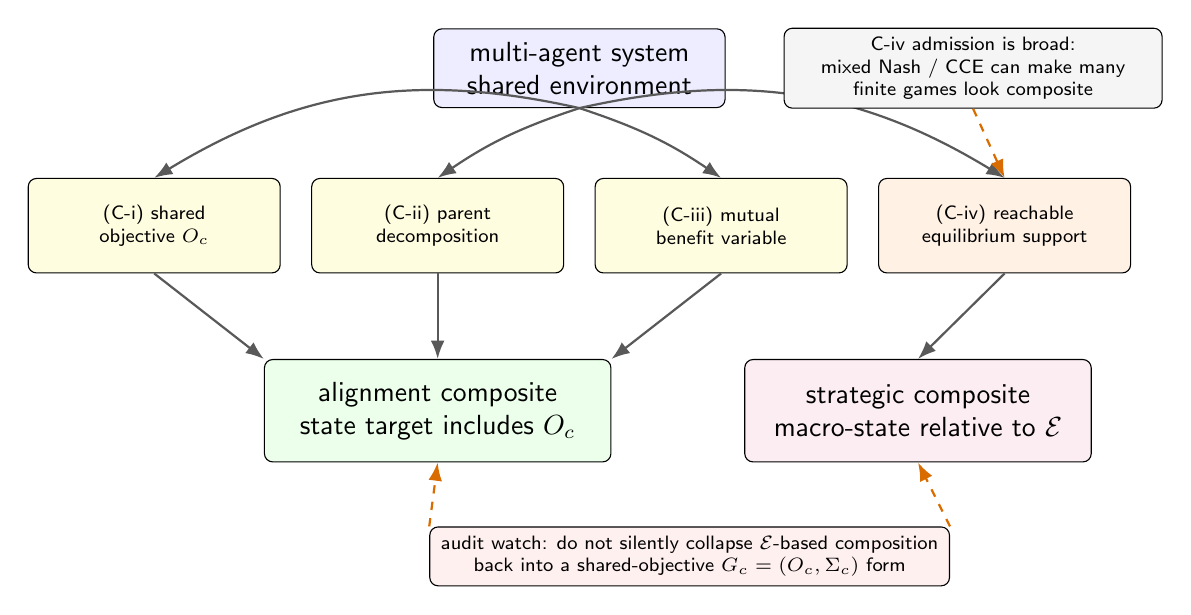
\begin{tikzpicture}[
  font=\sffamily,
  box/.style={draw, rounded corners=3pt, align=center, minimum width=37mm, minimum height=10mm, fill=white},
  route/.style={draw, rounded corners=3pt, align=center, font=\sffamily\scriptsize, minimum width=32mm, minimum height=12mm, fill=yellow!12},
  compout/.style={draw, rounded corners=3pt, align=center, minimum width=44mm, minimum height=13mm},
  note/.style={draw, rounded corners=3pt, align=center, font=\sffamily\scriptsize, fill=white},
  arrow/.style={-Latex, thick, draw=black!65},
  warn/.style={-Latex, thick, dashed, draw=orange!85!black}
]

\node[box, fill=blue!7] (multi) at (0,3.35)
  {multi-agent system\\shared environment};

\node[route] (c1) at (-5.4,1.35)
  {(C-i) shared\\objective $O_c$};
\node[route] (c2) at (-1.8,1.35)
  {(C-ii) parent\\decomposition};
\node[route] (c3) at (1.8,1.35)
  {(C-iii) mutual\\benefit variable};
\node[route, fill=orange!10] (c4) at (5.4,1.35)
  {(C-iv) reachable\\equilibrium support};

\draw[arrow] (multi.south) to[bend right=22] (c1.north);
\draw[arrow] (multi.south) to[bend right=8] (c2.north);
\draw[arrow] (multi.south) to[bend left=8] (c3.north);
\draw[arrow] (multi.south) to[bend left=22] (c4.north);

\node[compout, fill=green!8] (align) at (-1.8,-1.0)
  {alignment composite\\state target includes $O_c$};
\node[compout, fill=purple!7] (strat) at (4.3,-1.0)
  {strategic composite\\macro-state relative to $\mathcal E$};

\draw[arrow] (c1.south) -- (align.north west);
\draw[arrow] (c2.south) -- (align.north);
\draw[arrow] (c3.south) -- (align.north east);
\draw[arrow] (c4.south) -- (strat.north);

\node[note, fill=red!6, minimum width=66mm] (warn) at (1.4,-2.85)
  {audit watch: do not silently collapse $\mathcal E$-based composition\\back into a shared-objective $G_c=(O_c,\Sigma_c)$ form};
\draw[warn] (warn.north west) -- (align.south);
\draw[warn] (warn.north east) -- (strat.south);

\node[note, fill=gray!8, minimum width=48mm] (over) at (5.0,3.35)
  {C-iv admission is broad:\\mixed Nash / CCE can make many\\finite games look composite};
\draw[warn] (over.south) -- (c4.north);

\end{tikzpicture}
\end{document}
